\documentclass[11pt]{article}

\usepackage[margin=1in]{geometry}
\usepackage[T1]{fontenc}
\usepackage{amsmath,amssymb,booktabs,array}
\usepackage{graphicx}
\usepackage[dvipsnames]{xcolor}
\usepackage{tikz}
\usetikzlibrary{arrows.meta,positioning,fit,backgrounds}
\usepackage[hidelinks]{hyperref}
\usepackage{enumitem}

\newcommand{\AP}{\mathrm{AP}}
\newcommand{\IoU}{\mathrm{IoU}}
\newcommand{\BEV}{\mathrm{BEV}}
\newcommand{\soft}{\mathrm{softmax}}

\title{Robust Cooperative LiDAR Perception with\
Uncertainty-Aware Fusion and Spatial TrackFormer Association}
\author{Progress Report}
\date{July 2026}

\begin{document}
\maketitle

\begin{abstract}
This report describes a cooperative 3D perception pipeline for OPV2V under
localization and communication noise. A PointPillars detector provides local
vehicle proposals, BELT-style evidential and covariance-aware fusion recovers
substantial accuracy under noise, and a spatial adaptation of TrackFormer
produces cross-agent object-association embeddings. On the official noisy
OPV2V test set, uncertainty-aware BELT fusion improves $\AP@0.7$ from $0.294$
for corrected naive late fusion to $0.415$. Adding the current TrackFormer
association improves strict localization further to $0.423$, while slightly
reducing $\AP@0.5$; this identifies association recall as the main remaining
bottleneck.
\end{abstract}

\section{Problem and Motivation}

Cooperative perception lets several connected autonomous vehicles (CAVs)
share detections so that an ego vehicle can see beyond its own occlusions.
Late fusion is attractive because agents transmit compact object-level
messages rather than dense feature maps. Its weakness is that detections from
different agents must be expressed in a common coordinate frame, associated
correctly, and fused despite localization error and asynchronous observations.

We study PointPillars late fusion on the OPV2V benchmark~\cite{opv2v}. The
noise setting follows the BELT-Fusion repository: $0.2\,$m Gaussian position
noise, $0.2^\circ$ heading noise, and $100\,$ms communication delay. The
research questions are: (i) can uncertainty-aware fusion recover detection
accuracy under this noise; and (ii) can learned cross-agent association
improve over geometry-only association?

\section{PointPillars and the BEV Representation}

Each CAV observes a raw LiDAR point cloud
$\mathcal{P}_i=\{(x,y,z,r)\}$ in its local coordinate system. PointPillars
partitions the ground plane into fixed XY cells; all points in the same cell,
over the full vertical range, form one \emph{pillar}~\cite{pointpillars}.
The pillar feature network applies a learned point-wise encoding and pooling
operation to produce one learned descriptor for every nonempty pillar. These
descriptors are scattered back onto an XY grid and processed by a 2D
convolutional BEV backbone.

For our PointPillars configuration, the backbone output is
\begin{equation}
  F_i \in \mathbb{R}^{384\times100\times176}.
\end{equation}
The $100\times176$ dimensions are the backbone's spatial BEV grid after its
convolutional downsampling/upsampling design; they are not the raw LiDAR
point count. The $384$ channels are learned feature channels, formed by
concatenating three $128$-channel backbone branches. Detection heads applied
to $F_i$ predict vehicle boxes, orientations, confidence scores, and dense
anchor outputs.

For a predicted box $b_{i,k}$, let $\mathcal{R}_{i,k}$ be the set of BEV
backbone cells covered by its rotated footprint. The first embedding baseline
used only one $384$-D cell selected at the proposal anchor. The improved cache
retains \emph{all} cells $\{F_i(r):r\in\mathcal{R}_{i,k}\}$, typically
6--21 cells, plus their relative locations, the box, confidence, matched
ground-truth identity, and the agent transformation matrix. Importantly, BEV
features remain local to each agent; it is the predicted box geometry that is
transformed to the ego frame before cross-agent geometric comparison.

\begin{figure*}[t]
\centering
\resizebox{\textwidth}{!}{%
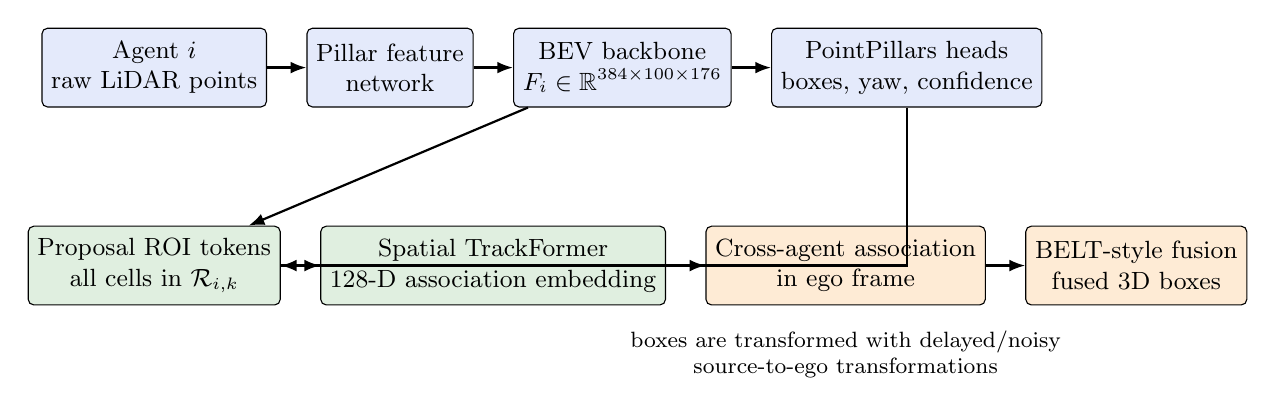
\begin{tikzpicture}[
  font=\small,
  box/.style={draw, rounded corners=2pt, align=center, minimum height=10mm,
              minimum width=19mm, fill=#1!14},
  arrow/.style={-{Latex[length=2mm]}, thick},
  node distance=8mm and 5mm
]
\node[box=RoyalBlue] (lidar) {Agent $i$\\raw LiDAR points};
\node[box=RoyalBlue, right=of lidar] (pillars) {Pillar feature\\network};
\node[box=RoyalBlue, right=of pillars] (bev) {BEV backbone\\$F_i\in\mathbb{R}^{384\times100\times176}$};
\node[box=RoyalBlue, right=of bev] (det) {PointPillars heads\\boxes, yaw, confidence};

\node[box=ForestGreen, below=15mm of lidar] (roi) {Proposal ROI tokens\\all cells in $\mathcal{R}_{i,k}$};
\node[box=ForestGreen, right=of roi] (tf) {Spatial TrackFormer\\128-D association embedding};
\node[box=BurntOrange, right=of tf] (assoc) {Cross-agent association\\in ego frame};
\node[box=BurntOrange, right=of assoc] (belt) {BELT-style fusion\\fused 3D boxes};

\draw[arrow] (lidar) -- (pillars);
\draw[arrow] (pillars) -- (bev);
\draw[arrow] (bev) -- (det);
\draw[arrow] (bev) -- (roi);
\draw[arrow] (det.south) |- (roi.east);
\draw[arrow] (roi) -- (tf);
\draw[arrow] (tf) -- (assoc);
\draw[arrow] (assoc) -- (belt);

\node[align=center, font=\footnotesize, below=2mm of assoc]
{boxes are transformed with delayed/noisy\\source-to-ego transformations};
\end{tikzpicture}
}
\caption{Implemented cooperative-perception pipeline. Each agent extracts
local BEV features and detections. Spatial TrackFormer converts all
vehicle-covered BEV cells into an association embedding, while BELT-style
fusion uses uncertainty to combine associated boxes.}
\label{fig:pipeline}
\end{figure*}

\section{Coordinate Alignment and Noise}

Let $T_{e\leftarrow i}\in SE(3)$ transform a source agent's local coordinates
into the ego frame. For a local proposal box, the center and yaw are aligned
before association as
\begin{equation}
  \tilde b_{i,k}^{(e)} = T_{e\leftarrow i}^{\mathrm{noisy,delayed}}\,b_{i,k}.
\end{equation}
The delayed/noisy transform is essential: a prior OpenCOOD late-fusion path
retained source boxes but used a clean transformation matrix during fusion,
thereby bypassing the intended pose perturbation. We corrected this path so
non-ego boxes are placed using the delayed, noisy pose.

This correction produces the valid robustness baseline: clean late fusion has
$\AP@0.7\approx0.78$, whereas noisy naive late fusion has $\AP@0.7=0.294$.
The drop is expected: small pose errors are amplified at high IoU because
several agents' boxes no longer align precisely.

\section{BELT-Style Uncertainty-Aware Late Fusion}

The public BELT-Fusion snapshot documents the method but does not provide a
complete runnable OPV2V/PointPillars path or released trained weights. We
therefore implemented an OpenCOOD-compatible adapter that retains the
published design principles~\cite{beltfusion}: evidential classification
uncertainty, heteroscedastic box uncertainty, uncertainty-aware confidence
fusion, and covariance-weighted box fusion.

For classification, an evidential head predicts nonnegative evidence
$e_c$ and Dirichlet parameters $\alpha_c=e_c+1$. The total evidence
$S=\sum_c\alpha_c$ determines an uncertainty proxy $u\propto 1/S$: low
evidence yields high uncertainty. For regression, the head predicts a
diagonal covariance $\Sigma_{i,k}$ for box parameters. Associated box
estimates are combined by precision weighting,
\begin{equation}
  \Sigma_f^{-1}=\sum_i \Sigma_i^{-1},\qquad
  \mu_f=\Sigma_f\sum_i\Sigma_i^{-1}\mu_i,
\end{equation}
so an uncertain observation has less influence on the fused box. The
implementation additionally accounts for known source pose-noise variance in
the ego frame.

This works because localization noise is not equally reliable across all
detections. Rather than averaging inconsistent boxes uniformly, the fusion
stage downweights detections whose learned or propagated uncertainty is high.

\section{From Temporal TrackFormer to Spatial Association}

Original TrackFormer solves multi-object tracking as frame-to-frame set
prediction~\cite{trackformer}. A CNN extracts image features, a Transformer
encoder forms image memory, and a decoder uses object queries. Object queries
from frame $t-1$ are propagated into frame $t$; Hungarian matching, class/
no-object supervision, $\ell_1$ box loss, generalized-IoU loss, and
false-positive track-query supervision train the system jointly.

Our setting replaces temporal dependence with a spatial one at a common
timestamp. A source CAV plays the role of the previous frame and the ego CAV
plays the role of the current frame. The model consumes PointPillars ROI tokens
instead of image features, propagates source-object queries to the ego BEV
memory, and asks whether source and ego proposals describe the same physical
object. This is an adaptation of TrackFormer's attention and query-propagation
mechanism; it is not a claim that the original paper performed V2X association.

For proposal $k$, ROI tokens are projected and position encoded before the
encoder/decoder. The final query $q_{i,k}$ is combined with explicit ego-frame
box geometry $g_{i,k}$ and confidence $s_{i,k}$ to form a normalized
association embedding,
\begin{equation}
 z_{i,k} = \frac{h_\theta([q_{i,k};g_{i,k};s_{i,k}])}
 {|h_\theta([q_{i,k};g_{i,k};s_{i,k}])|_2}\in\mathbb{R}^{128}.
\end{equation}
The association loss includes an identity contrastive term and hard-negative
term,
\begin{equation}
 \mathcal{L}_{\mathrm{assoc}} =
 \lambda_{\mathrm{emb}}\mathcal{L}_{\mathrm{InfoNCE}}+
 \lambda_{\mathrm{hard}}\mathcal{L}_{\mathrm{hard}},
\end{equation}
where hard negatives are nearby vehicles with similar physical size. During
full TrackFormer training, this is combined with detection/tracking losses,
\begin{equation}
 \mathcal{L}_{\mathrm{full}}=\mathcal{L}_{\mathrm{assoc}}+
 \mathcal{L}_{\mathrm{cls}}+\lambda_1\mathcal{L}_{\ell_1}+
 \lambda_{\mathrm{giou}}\mathcal{L}_{\mathrm{GIoU}}.
\end{equation}

The explicit geometry is necessary because BEV appearance alone is ambiguous:
nearby vehicles often have similar LiDAR structure. The transformer supplies
object and surrounding spatial context, while ego-frame geometry and
confidence provide calibrated physical constraints.

\section{Experimental Results}

All end-to-end AP results below use the official OPV2V test split and the
same noise realization. Values are shown to three decimal places.

\begin{table}[h]
\centering
\caption{Noisy OPV2V late-fusion results.}
\label{tab:ap}
\begin{tabular}{lccc}
\toprule
Method & $\AP@0.3$ & $\AP@0.5$ & $\AP@0.7$ \\
\midrule
Naive late fusion & 0.860 & 0.712 & 0.294 \\
BELT geometry fusion & 0.851 & \textbf{0.752} & 0.415 \\
BELT + Spatial TrackFormer & 0.846 & 0.743 & \textbf{0.423} \\
\bottomrule
\end{tabular}
\end{table}

The geometry-conditioned association head reached $0.915$ top-1 cross-agent
association accuracy on clean validation and $0.891$ on the clean official
test set. Without retraining, it retained $0.907$ top-1 accuracy on noisy
validation. A noisy association-head fine-tuning stage achieved $0.909$ on
noisy validation, but did not yield a meaningful additional end-to-end test
gain; the best test result remained $\AP@0.7=0.423$.

BELT provides the dominant robustness recovery: $0.294\rightarrow0.415$ at
$\AP@0.7$. TrackFormer adds a smaller but held-out improvement:
$0.415\rightarrow0.423$. The trade-off is association recall: TrackFormer
forms $8.94$ multi-agent groups per frame compared with $10.16$ for
geometry-only BELT, which explains the small $\AP@0.5$ reduction.

\section{Conclusions and Next Steps}

The experiments establish a valid noisy PointPillars baseline, a working
uncertainty-aware BELT implementation, and a cross-agent spatial TrackFormer
association model with strong standalone identity accuracy. The remaining gap
is not simply embedding quality: an embedding top-1 score does not directly
optimize the precision--recall trade-off of complete fusion groups.

The next step is to evaluate association links directly against ground-truth
identities on noisy validation scenes, measuring false links and missed links
separately. These diagnostics can train a calibrated pairwise association
score that jointly uses embedding similarity, ego-frame displacement,
predicted covariance, and confidence, followed by one-to-one global
assignment. This targets the observed failure mode: recover valid groups
without reintroducing incorrect noisy associations.

\begin{thebibliography}{9}

\bibitem{opv2v}
R.~Xu, H.~Xiang, X.~Xia, X.~Han, J.~Li, and J.~Ma,
``OPV2V: An Open Benchmark Dataset and Fusion Pipeline for Perception with
Vehicle-to-Vehicle Communication,'' in \emph{IEEE ICRA}, 2022.

\bibitem{pointpillars}
A.~H.~Lang, S.~Vora, H.~Caesar, L.~Zhou, J.~Yang, and O.~Beijbom,
``PointPillars: Fast Encoders for Object Detection from Point Clouds,''
in \emph{CVPR}, 2019.

\bibitem{trackformer}
T.~Meinhardt, A.~Kirillov, L.~Leal-Taix\'{e}, and C.~Feichtenhofer,
``TrackFormer: Multi-Object Tracking with Transformers,'' in \emph{CVPR},
2022.

\bibitem{beltfusion}
Z.~Zhao, C.~Zhao, K.~Chen, Y.~Ji, and Y.~Du,
``BELT-Fusion: Bayesian Evidential Late Fusion for Trustworthy V2X
Perception,'' \emph{IEEE Transactions on Intelligent Transportation
Systems}, 2025.

\end{thebibliography}

\end{document}
